\documentclass[conference]{IEEEtran}
\IEEEoverridecommandlockouts
% The preceding line is only needed to identify funding in the first footnote. If that is unneeded, please comment it out.
\usepackage{cite}
%\usepackage{}
\usepackage{amsthm}
\usepackage{amsmath, amssymb,amsfonts}
\usepackage{algorithmic}
\usepackage{graphicx}
\usepackage{textcomp}
\usepackage{xcolor}


\theoremstyle{definition}
\newtheorem{definition}{Definition}
%\usepackage{CJK}

\def\BibTeX{{\rm B\kern-.05em{\sc i\kern-.025em b}\kern-.08emz
    T\kern-.1667em\lower.7ex\hbox{E}\kern-.125emX}}
\begin{document}

\title{Finding Influential Users in Twitter: Model Identification from Topic-Sensitive TwitterRank\\
% {\footnotesize \textsuperscript{*}Note: Sub-titles are not captured in Xplore and
% should not be used}
% \thanks{Identify applicable funding agency here. If none, delete this.}
} 
\author{\IEEEauthorblockN{1\textsuperscript{st} Yanxiao Liu}
	\IEEEauthorblockA{\textit{School of Science and Engineering} \\
		\textit{The Chinese University of Hong Kong, Shenzhen}\\
		Shenzhen China \\
		liuyanxiao712@hotmail.com}
	\and
	\IEEEauthorblockN{2\textsuperscript{nd} Jiayuan Li}
	\IEEEauthorblockA{\textit{School of Science and Engineering} \\
		\textit{The Chinese University of Hong Kong, Shenzhen}\\
		Shenzhen China \\
		117010120@link.cuhk.edu.cn}
	\and
	\IEEEauthorblockN{3\textsuperscript{rd} Yuji Cao}
	\IEEEauthorblockA{\textit{School of Science and Engineering} \\
		\textit{The Chinese University of Hong Kong, Shenzhen}\\
		Shenzhen China \\
		117010007@link.cuhk.edu.cn}
}

\maketitle

\begin{abstract}
Directed links in social media network can represent relationships and be used to determine a user's influence on others. User influence is a crucial concept in sociology and viral marketing for its role in the trend formation, but common methods such as PageRank alogorithm fail to adapt to the change of topics, which should be considered in certain topics since users in different fields have different influence, to make precise assessment. This paper focuses on the problem of identifying influential users of one popular social network, Twittter. Based on the large amount of data collected from Twitter, we present two metrics to measure the importance of users' ranks: TwitterRank ranking on topic-similarity and topology (link structure), and expertness ranking on if it's professional in specific topic. Finally, we balance the two rankings by Borda count and obtain a model to predict the rank of real movies' popularity. The detailed evaluation has also been used to measure the model's performance. Results show that our modified TwitterRank outperforms the classic PageRank algorithm on influence measurement of a certain topic, and may be useful in the future for more precise measurement.
\end{abstract}

\begin{IEEEkeywords}
Twitter, influential nodes, social network, topic-sensitive.
\end{IEEEkeywords}



\section{Introduction}

Influence has long been studied in the fields of sociology, communication, marketing, and political science (Rogeers 1962; Katz and Lazarsfeld 1955). Studying influence of users and their messages can help us better understand why certain trends or innovations are adopted faster than others and how we could learn the truths in reality by analyzing the social responding. 

Micro-blogging is an emerging form of communication boomed in current times. It
provides a platform that allows users to publish brief message updates. Popular
topics will always be discussed on some micro-blogging platforms. One of the most notable micro-blogging services is \textit{Twitter}. \textit{Users} can publish \textit{tweets}, which makes \textit{Twitter} provides the "social-networking" functionality.(Juhi, Farshad, Ashkan, Krishna, 2012) Unlike other social network services that require users to grant friend links to other users befriending them, \textup{Twitter} employs a social-networking model called "following", in which each \textup{user} is allowed to choose who she wants to follow without seeking any permission. Conversely, she may also be followed by others without granting permission first. 

In this report we are interested in identifying the influential \textup{users}
on the specific topic and investigate their messages with influence in the real
world. The benefit of solving this problem is multifold. First, it potentially
brings order to the real-time web in that it allows the search results to be
sorted by the authority/influence of the contributing \textup{users}. Second, by investigating their messages' influence it could lead to analyze the rationality and reasons behind the real-world phenomenon. At last identifying influential \textup{users} for certain topics can improve the quality of the opinions gathered.(Kwak, Lee, Park, Moon, 2010)

In current studies \textup{Twitter} and many other applications interpret a \textup{user's} influence as the number of followers she has. However, is this really a good indicator of influence? First, the “following” relationship is so casual that each \textup{user} just randomly follows someone, and those being followed follow back just for the sake of courtesy.(Welch, Schonfeld, He, Cho, 2011) Second, when it's analyzing node importance in a social network topology, it may result in the general influence. But when researchers study opinions gathering and information flow, it's more likely to need to study importance in a specific topic. A node with general importance may not have same importance in every field. 

In this project we have made two contributions. First, we implement the algorithm called TwitterRank to measure the topic-sensitive influence of the \textup{users}. This metric is an extension of the famous Google PageRank algorithm and can be used to investigate the influential users in a network about a specific topic. Second, we identify among different factors of measurement which one is the most decisive and its connection with other factors. 

The rest of this report is organized as follows: Two \textup{Twitter} datasets
have been prepared for the purpose of this study. Section 2 describes in detail how the datasets are prepared. The methodologies of TwitterRank ranking, expertness ranking and how are these two combined with another is elaborated in Section 3. Based on these ranking methods, the model identification is proposed to measure the real rank of movies' popularity in Section 4. Section 5 presents the evaluation of our model. Finally, Section 6 concludes with openness for further research. 



\section{Twitter Dataset}
\subsection{Data Collection}
For the purpose of this study, a set of Twitter data about film reviews was prepared in July, 2019 as follows:

\begin{itemize}
	\item We crawl a sets of 500 \textup{tweets} which contain the key words as the training set. The keywords are the names of several movies opened on 12th July 2019.
	
	\item We trace back to obtain two set of users who have published those \textup{tweets}.
	
	\item We then crawl all the \textup{followers} and \textup{friends} of each individual \textup{user} $s$ and store them in a set $S$.
	
	\item For each $s$ in set $S$, we obtain the number of \textup{tweets} published by each one of $s$'s friends. Denote the set of all the tweets obtained so far as $\tau$.
\end{itemize}

\subsection{Topic Distillation}\label{AA}
To distill the topics that \textup{users} are interested in, we should naturally focus on \textup{tweets}. The need to focus on the number of users and the number of topics. We form a matrix: 

\begin{itemize}
	\item $DT$, a $D$ $\times$ $T$ matrix, where $D$ is the number of \textup{users} and $T$ is the number of topics. $DT_{ij}$ contains the number of times a word in \textup{user} $s_i$'s \textup{tweets} has bee nassigned to topic $t_j$.
\end{itemize}


\section{Methodologies for identifying influential users}
\subsection{Background}
There are a number of different ideas and theories about how to detect the important nodes in a network. Studies in this topic is significant because identifying influential ones can be applied in a large amount of fields, like marketing, technology and economics. The information flow has been studied through years. The influence of links and nodes in a network is one most significant factor of the network, which decides the function and performance of it.(Ghosh, Viswanath, Kooti, Sharma, Korlam, Benevenuto, 2012)

The traditional view assumes a minority of members in a society makes them exceptionally persuasive in spreading ideas to others. When people want to identify these influential minorities, normally people assume the more people connect with them, the more they are important. This is called indegree method and have been used widely: eg. Google's PageRank.(Cha, Haddadi, Rebevenuto, Gummadi, 2010) However, this method and similar ones are not topic-sensitive, which means it have same performance through different topics.

However, when it need to be applied in a specific field, the detecting method should be sensitive to this certain topic, since people always have different important in different fields. So the topic-sensitive one, TwitterRank algorithm that we are implementing is to solve this problem. 

\subsection{TwitterRank Ranking}
Intuitively, the influence of a \textup{user} is similar with the "authority" of a web page. This similarity motivates the use of PageRank in measuring influence. But there are still differences between them: The influence on each follower is purely based on relative amount of content the follower receives as the latter may not read content with topics less interesting even when the relative content is large. Since users generally have different expertise and/or interests in various topics, influence of users also vary in different topics. Given this, a topic-sensitive TwitterRank is proposed to measure the influence of users. 

After topic distillation the matrix $DT$ contains the number of times a word in a \textup{twittere's tweets} has been assigned to a particular topic. The normalization can be implemented as $DT'$ such that $||DT'_i|| = 1$ for each row $DT'_i$. 

At first we form a directed graph $D(V, E)$ with the \textup{users} and the “following” relationships among them. $V$ is the vertex set, which contains all the \textup{users}. $E$ is the edge set. There is an edge between two \textup{users} if there is “following” relationship between them, and the edge is directed from \textup{follower} to \textup{friend}.

Different from the original PageRank algorithm, we propose a \textup{random surfer model} on graph $D$ computes the TwitterRank as follows: the random surfer visits each \textup{user} with certain probability by following the appropriate edge in $D$. This random surfer performs a topic-specific random walk and then we could contruct a topic-specific relationship network among \textup{users}. 

\theoremstyle{definition}
\begin{definition}{Transition Probability}
	Given a topiv t, each element of matrix $P_t$, $i.e.$ the transition probability of the random surfer from follower $s_i$ to friend $s_j$, is defined as:
	
	\begin{align}
	P_t(i,j) = \frac{|\tau_j|}{\sum_{a: \, s_i \,\, follows \,\, s_a}|\tau_a|} * sim_t(i,j)
	\end{align}
	
	where $|\tau_j|$ is number of tweets published by $s_j$, and $\sum_{a: \, s_i \,\, follows \,\, s_a}|\tau_a|$ sums up the number of tweets published by all of $s_i$'s friends. 
	
	$sim_t(i,j)$ is the similarity between $s_i$ and $s_j$ in topic $t$:
	
	\begin{align}
	sim_t(i,j) = 1 - |DT'_{it} - DT'_{jt}|
	\end{align}
\end{definition}

The calculation metric of transition probabilities can be understood in this way: For a \textup{twitter} $s_i$, the more one his friend $s_j$ publishes, the higher portion of tweets $s_i$ reads is from $s_j$. Then generally this leads to a higher transition probability from $s_i$ to $s_j$. 


\begin{figure}[htb]
\centerline{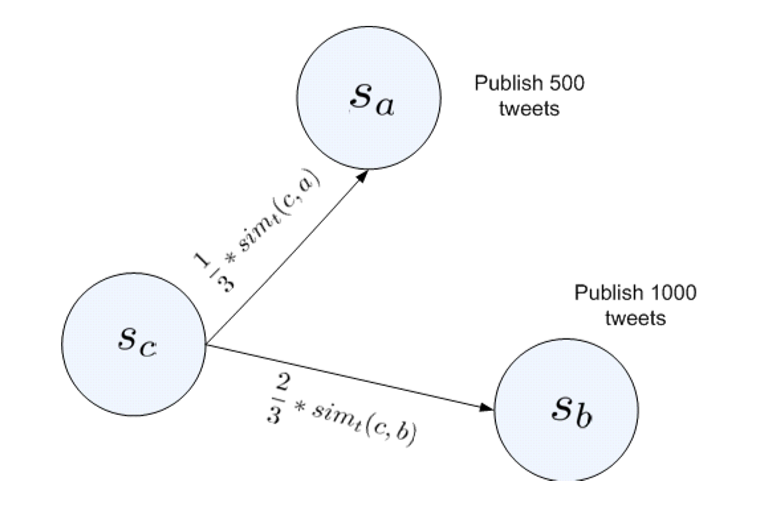
\includegraphics{twitterers.png}}
\caption{Similarity figure}
\label{fig}
\end{figure}


The similarity is important. A row $DT'_j$ contains the probability of user $s_j$’s interest in different topics. The similarity between $s_i$ and $s_j$ in topic $t$ can be evaluated as the difference between the probability that the two users are interested in the same topic $t$, which is basically the second term in the RHS of $Eq.(3)$. The more similar the two users are, the higher the transition probability from $s_i$ to $s_j$.



\theoremstyle{definition}
\begin{definition}{teleportation vector}
	The teleportation vector of the random surfer in topic t is defined as: 
	
	\begin{align}
	E_t = DT''_t
	\end{align}
	
	$DT''_t$ is the t-th column of matrix $DT''$, which is the column-normalized form of matrix DT such that $||DT''_t|| = 1$. 
	
	
\end{definition}


With the transition probability matrix and teleportation vector defined, the topic-specific \textup{TwitterRank} can be calculated.



\theoremstyle{definition}
\begin{definition}{topic-specific TwitterRank}
	The topic-specific TwitterRank of the users in topic t, denoted as $\vec{TR_t}$, can be calculated iteratively by:
	
	\begin{align}
	\vec{TR_t} = \gamma R_t \times \vec{TR_t} + (1 - \gamma)R_t
	\end{align}
	
	where $\gamma$ is a parameter between 0 and 1 to control the probability of teleportation. The lower $\gamma$ is, the higher probability the random surfer will teleport to users according to $E_t$, and vice versa. 
	
\end{definition}


\subsection{Expertness Ranking}

Except for the number of tweets a user has sent and the topic similarity between he and his follower, his influence in a specific topic is also related to his \textit{expertness} in this topic. For example, you may follow your friend Bob who is a filmaholic, sending 10 tweets about movie everyday. However, he may not be as influential as Steven Spielberg or a professional movie critic who only sends 1 or 2 tweets everyday, but containing their experience and a deeper understanding of movie.

To solve this problem, we introduce the measurement of \textit{retweet} to quantify the expertness of the user in a specific area. 

\theoremstyle{definition}
\begin{definition}{Given a user $s_{i}$ and the number of retweets $R_{m}$ of his history tweets $m_{i}$ that are related to a topic, the expertness of this user can be calculated by:}

	\begin{align}
	B = \frac{\sum_{m_i\in M_i} R_m}{k} 
	\end{align}
	
	 where $M_i$ is the set of all history tweets published by user $i$ and $k$ is the total number of these history tweets.
\end{definition}

In general, the more retweets a tweet has, the wilder it will be spread and the more influential the user who sends this tweet will be. This method helps specialize the influence measurement in a specific topic, especially for users whose tweets have a lot more retweets in some topics than the others. This expertness serves as a certain kind of bias in the specific topic.

This equation is designed to use averaging instead of nummation in order to fit two common wisdoms: First, sending a lot of useless tweets with little retweets cannot make a user more influential. Second, a user with only 1 or 2 tweets really popular but a lot more unpopular does not necessarily means he is influential. In the case that he occasionally tweets a movie highly related to his experience, which makes the tweets more popular, he is only more "professional" in this movie instead of the movie topic. However, this indeed indicates that he is capable of understanding some of the movies, which correspondes to the averaged expertness he gains from this tweet. In all, averaging shows a more general condition of the tweets and the user, as well as avoiding the influence of incident points.


\subsection{Combination of two rankings}
From the above two measurements, we have already aquired two rankings: the \textit{TwitterRank} ranking and the \textit{Expertness} ranking. 

In order to obtain the final ranking, we adapt a variant of \textit{Borda Count} in voting, namingly \textit{Weighted Borda Count} to combine these two rankings, assuming they exert influence on the final ranking in the same scale or in linear structure like two individuals in the original Borda Count.

\begin{definition}{The final ranking based on the \textit{TwitterRank} ranking and the \textit{Expertness} ranking can be calculated by:}

	\begin{align}
	Ranking = \alpha(A_i-1)+\beta(B_i-1)
	\end{align}
	
	 where $\alpha$ and $\beta$ are the weights to be determined using training data, and $\alpha + \beta = 1$. $A_i$ and $B_i$ are the rankings of user i in \textit{TwitterRank} ranking and \textit{Expertness} ranking. 
\end{definition}

By balancing those two rankings to find the final result, we can find the coefficients of the range of them that can make the ranking fits the real rank best. We define the results are our model and then we can test the rank in following sections.




\section{Model Identification}
\subsubsection{Methodology}

In this section we use the first group, the training data to determine the coefficients $\alpha$ and $\beta$ in the final combined ranking, which fits the real ranking best. 

By the methodology of our TwitterRank and Expertness analysis, we have found two rankings. Our model are the coefficients that balance these two rankings to find the real ranking. The coefficients are studied about:


\begin{align}
Ranking = \alpha(A_i-1)+\beta(B_i-1)
\end{align}

where $\alpha$ and $\beta$ are the weights to be determined using training data, $A_i$ and $B_i$ are the rankings of user i in \textit{TwitterRank} ranking and \textit{Expertness} ranking. 

By ranging coefficients from 0.01 to 0.99, we could draw the ranking we have about those five movies: Then by calculating the penalty: the difference of each ranking position between the rank of movies we get and the real rank, we can find the range of coefficients that fit best:


\begin{figure}[htb] \centering
	\centerline{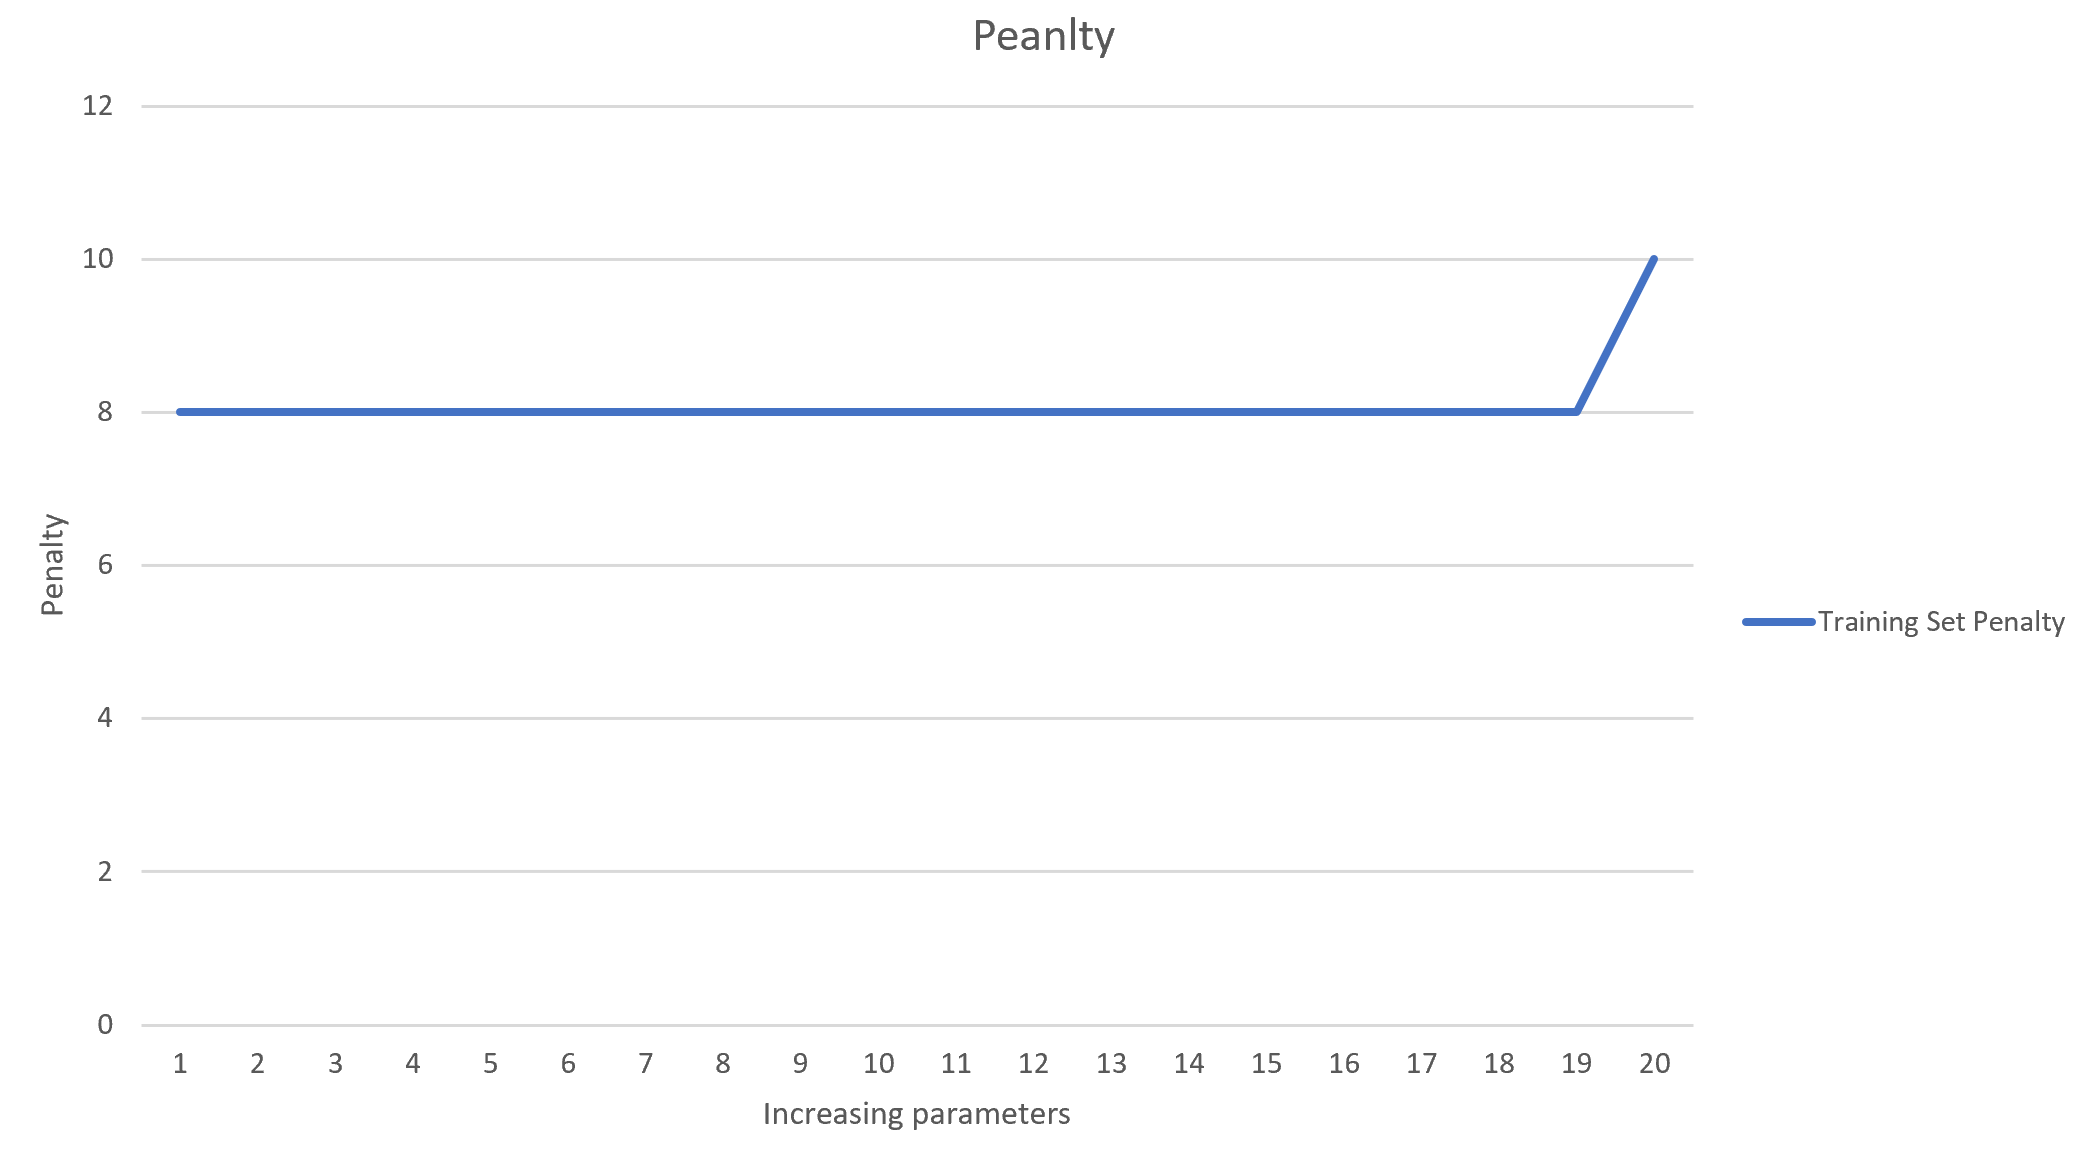
\includegraphics[width=0.8\linewidth]{c.png}}
	\caption{Training Set Penalty}
	\label{fig}
\end{figure}

From the results we can know when the coefficient $\alpha$ varies from 0 to 0.9, the penalty is always same. So then in the next step we are going to decide the coefficient in the next section. 

\section{Evaluation}
In the data collection part, we prepared two data sets, Training Set and Test
Set. To evaluate our model's performance, on the Training Set, we adjusted the
$\alpha$ and $\beta$ in the weighted Borda Count to find the coefficients which
make our model ranking more ``close'' to the actual ranking(the Box Office ranking). After finding such coefficients, we
tested them on the Test Set. The more ``close'' the ranking between two rankings,
the model is better. To evaluate the how ``close'' between the model
ranking and the actual ranking, we construct a function called \textit{penalty}
function. 
\begin{definition}{The \textit{penalty} between two rankings can be calculated by:}
	
	\begin{align}
	Penalty = \sum_{i\in I}{|M_i - A_i|}
	\end{align}
	
	where \textit{I} is the set of all the movies and \textit{i} is movie in the
	set, $M_i$ is the position of movie in the model ranking and $A_i$ is the
	position of each movie in the actual ranking.
	
\end{definition}

In general, the less the \textit{penalty} is, the better the model is. Also, the
\textit{penalty} function reflects the difference between our model ranking and
actual ranking, which just identifies the rank of these movies' popularity is
working well or not.

In Training Set and Test Set, the rank is regarding to (Shaft, Hampstead, Vault,
Head Count, Deep Murder) and (Crawl, Stuber, The Farewell, Bethany Hamiton,
Rojo), respectively. Also, above rankings are just the Box Office Rank of them.



%\begin{figure}[htb] \centering
%	\centerline{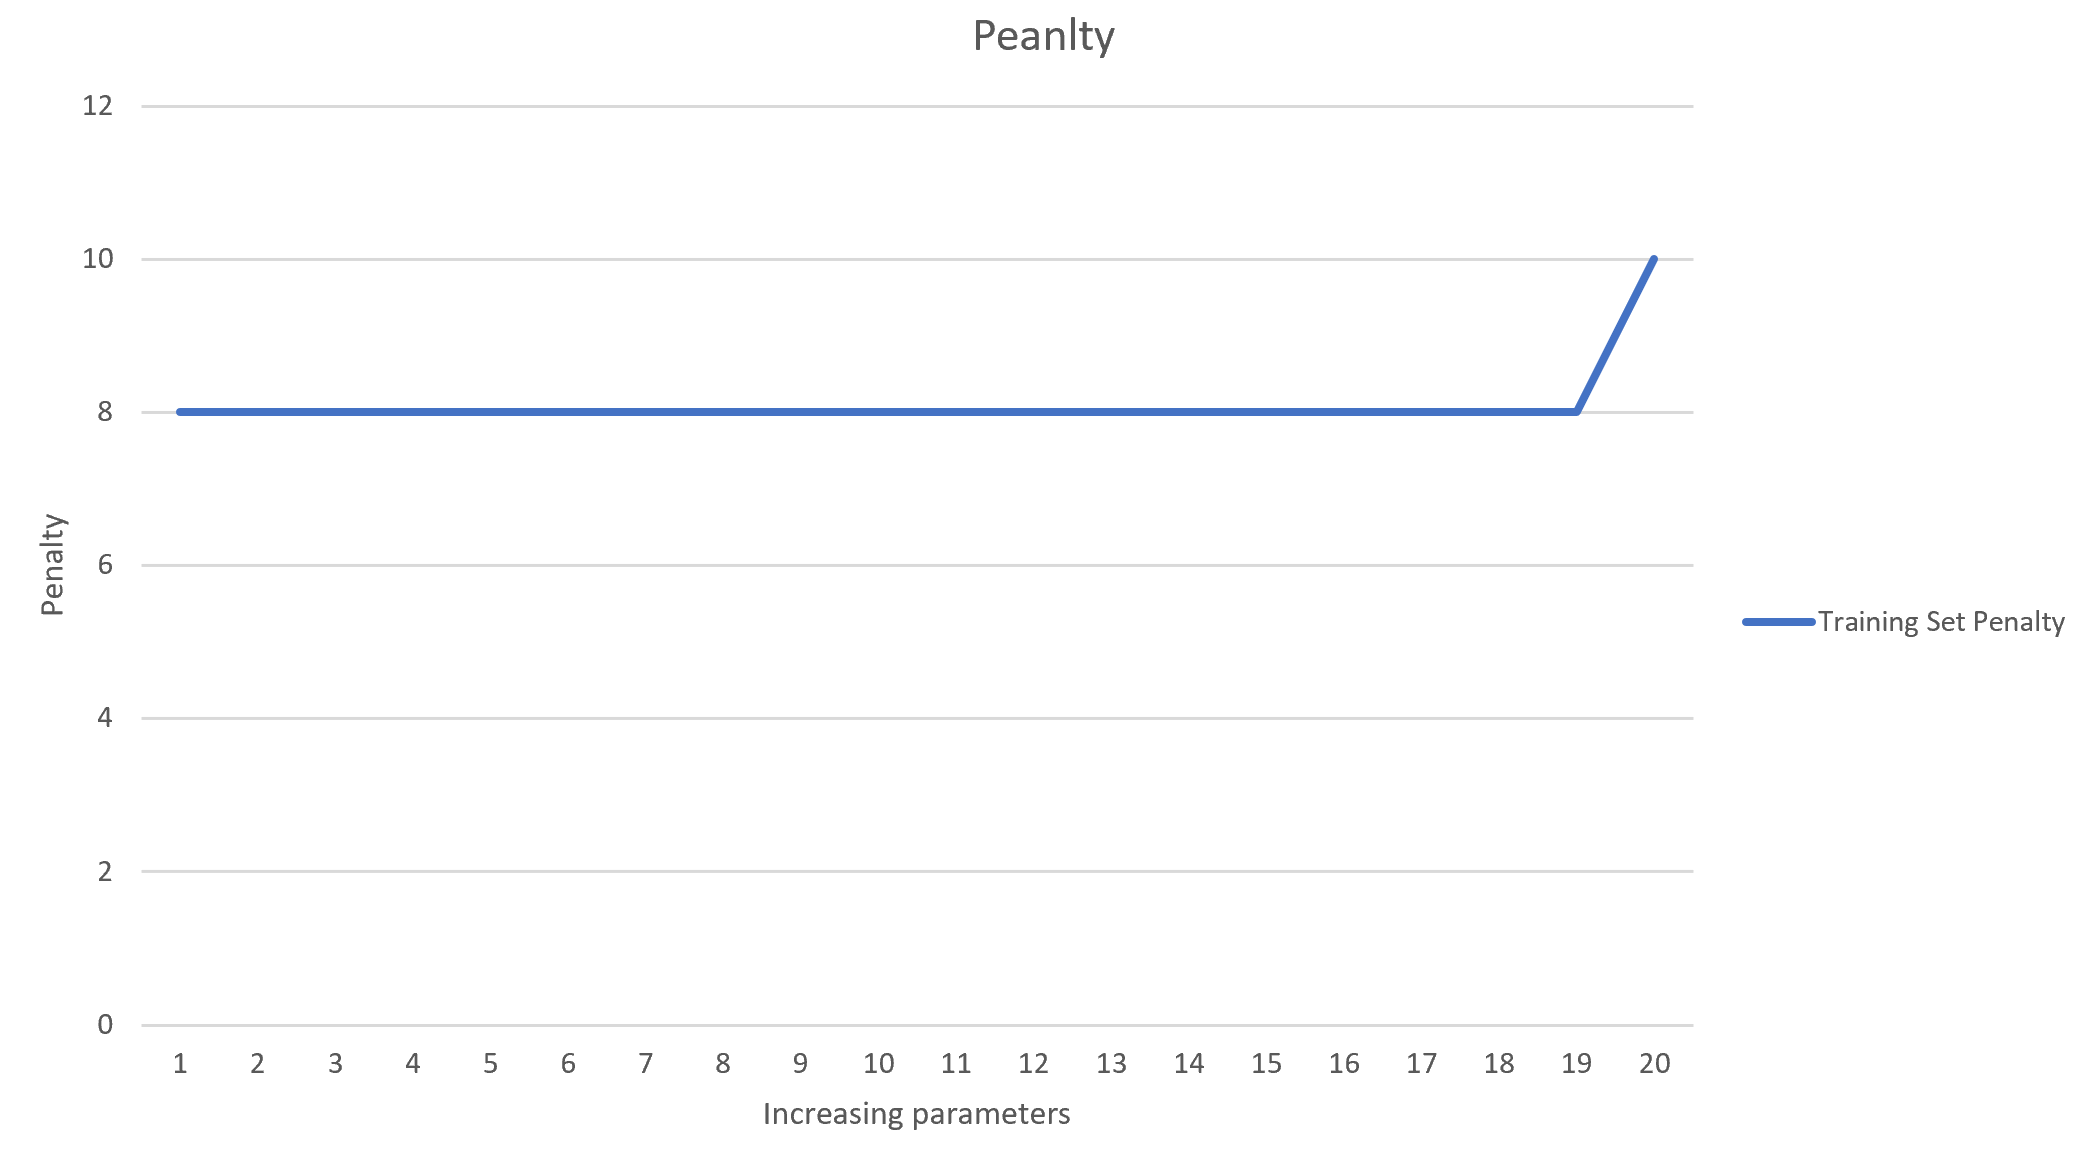
\includegraphics[width=0.8\linewidth]{c.png}}
%	\caption{Training set penalty}
%	\label{fig}
%\end{figure}


\begin{figure}[htb] \centering
	\centerline{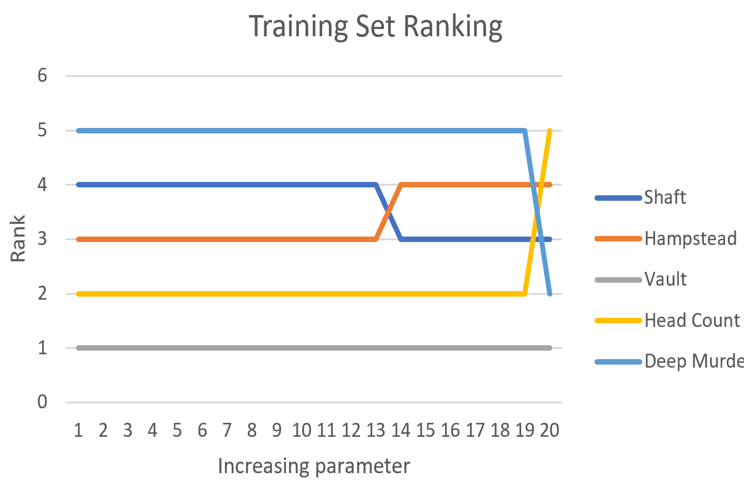
\includegraphics[width=0.8\linewidth]{training_rank.png}}
	\caption{Ranking of Training Set}
	\label{fig}
\end{figure}

\begin{figure}[htb]
	\centerline{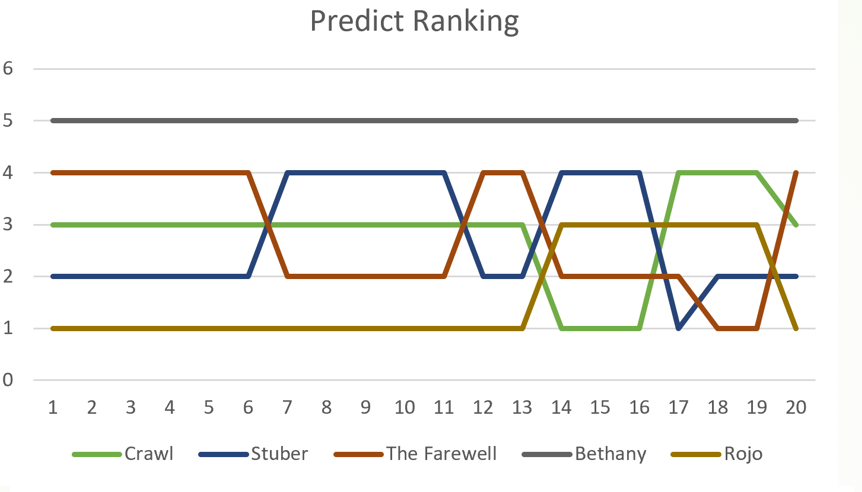
\includegraphics[width=0.8\linewidth]{test_rank.png}}
	\caption{Ranking of Test Set}
	\label{fig}
\end{figure}

In Figure 3, the x axis represents the \textit{TwitterRank} weight in the final
combined ranking, which is the 0.05 * increasing parameter. The y axis
represents each movie's rank in the final ranking with each coefficient
configuration. As illustrated in Figure 4, in general, as the \textit{TwitterRank}
weight increasing, the penalty drops. From our trail, we concluded the weight of
\textit{TwitterRank} with 0.73 is the most feasible one.

\begin{figure}[htb]
	\centerline{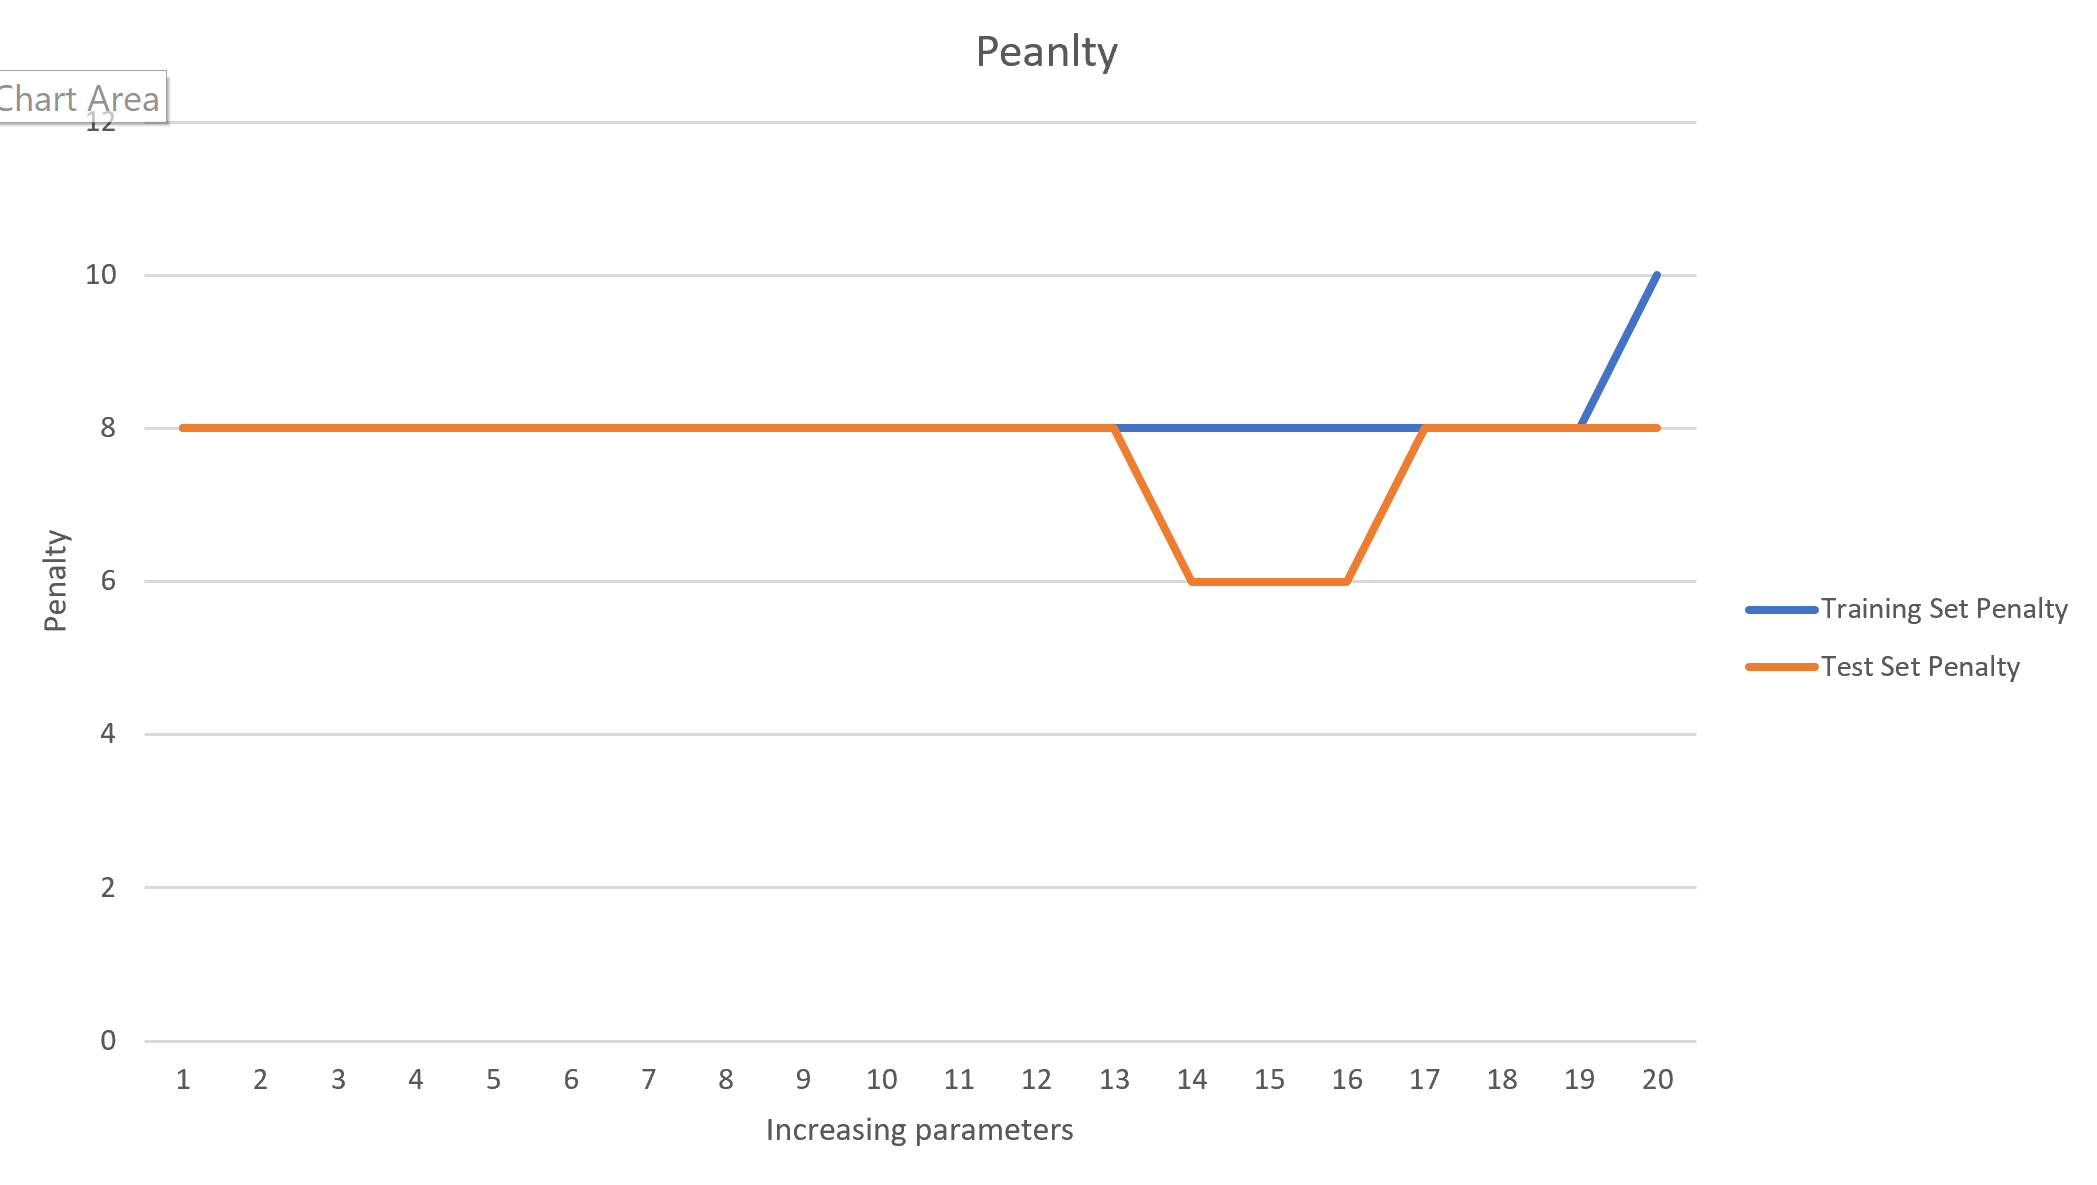
\includegraphics[width=0.8\linewidth]{penalty.jpg}}
	\caption{Penalty of Two Data Sets}
	\label{fig}
\end{figure}



Attaching it on the Test Set, as the results shown in Figure 5, we can see that
when the the weight of \textit{TwitterRank} is 0.73, the penalty is lower than
the others. This results shows that by analyzing the topic popularity in
Twitter, with 0.73 weight of \textit{TwitterRank} and 0.27 weight of
\textit{Expertness Rank}, this model can partially predict the movie's Box Office Rank.

\section{Ranking Analysis}
Section 5 predicts the movie ranking of the testing dataset by calculating the user infuence with our identified model, and evaluats our model using the penalty function. This section analyzes the results of the original PageRank method as well as our modified TwitterRank method, and obtains some insights regarding to the mechanism and the difference between them.

\subsection{Result comparison between ranking methods}
The graph of the partial ranking for first 30 users (sorted by name alphabetically) using two ranking methods is shown below.

\begin{figure}[htb]  
	\centering                       
	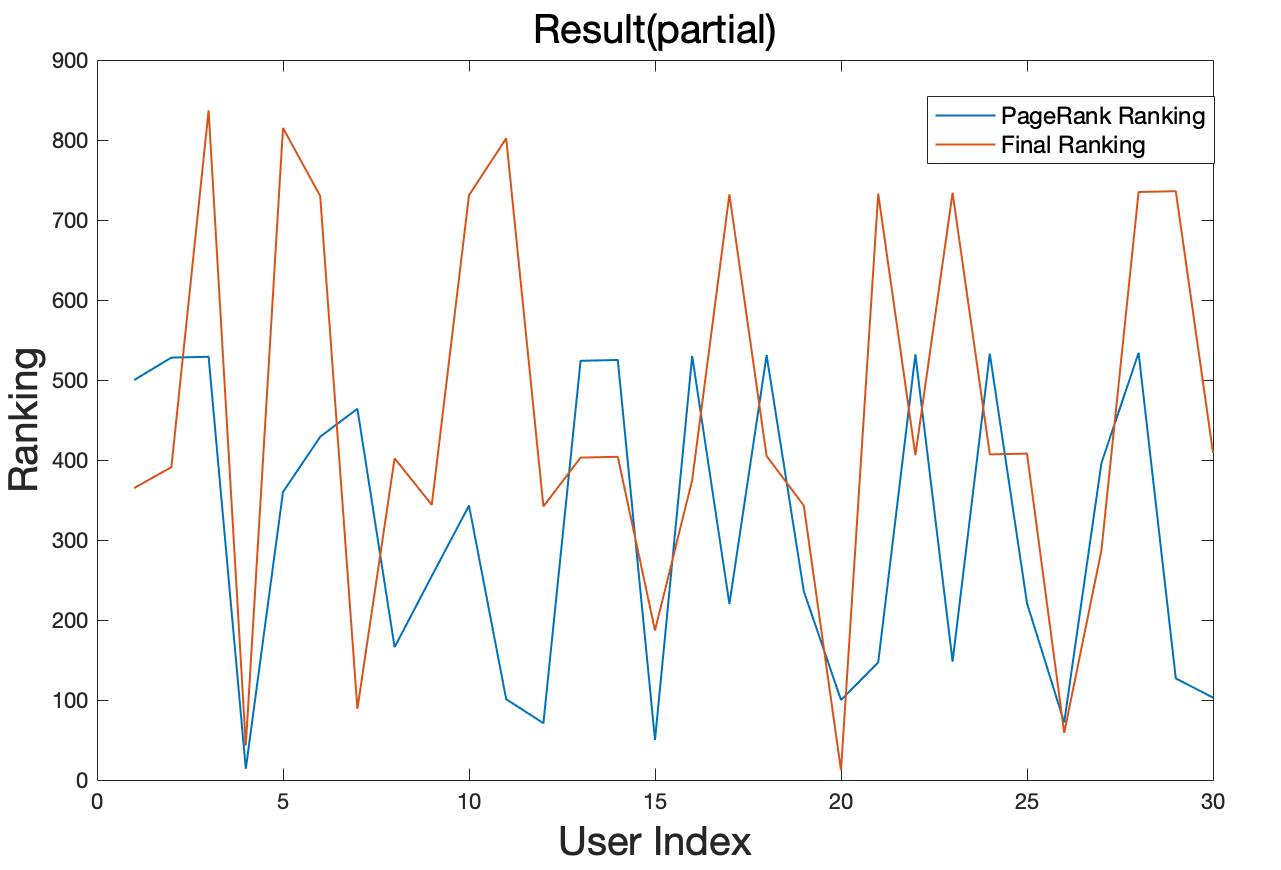
\includegraphics[width=0.8\linewidth]{2.png}
	\caption{User Ranking in Two Ranking Methods}
	\label{page-our}
\end{figure} 

The points on the blue curve represents the ranking of PageRank method, and the points on the red curve represents the ranking of our modified TwitterRank.\par From the graph above we can see that these two methods generates very different results: some users tend to have similar ranking, such as user 4; other users may have much lower rankings like user 10. And when we trace back to find their TwitterRank and Expertness ranking, we find that user 4 has a TwitterRank ranking of 35 and expertness ranking of 42 which are much closer to his PageRank ranking 14. However, user 10 has a very bad performace in his expertness ranking - ranking the last one, and we assumes that this results in the dramatic decrease of his final ranking. \par
From the finding above, we may reach our first conclusion that we do propose a topic-sensitive method that produce more accurate ranking in a specific topic than original the PageRank.


\subsection{Coefficients in the weighted Borda Count}
The graph of the final ranking with 4 different coefficients is shown below.

\begin{figure}[htb]  
	\centering                       
	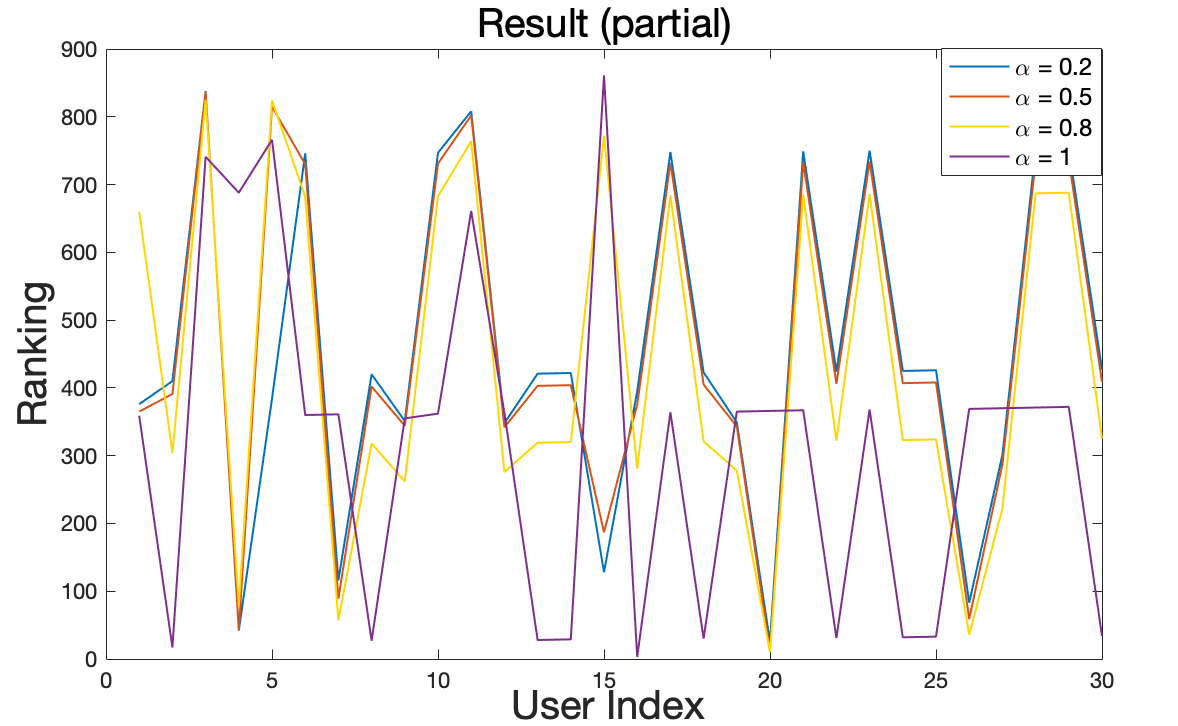
\includegraphics[width=0.8\linewidth]{3.png}
	\caption{Final rank with 4 different coefficients }
	\label{dif-co}
\end{figure} 

We can clearly see that different coefficients leads to different rankings, which means the TwitterRank ranking and the Expertness ranking do have their own and different effects on determining the influence of one iser and our algorithm seemingly make sense to combine two rankings.\par
Next then dive into two examples to analyze the relationship between these two rankings and the final ranking.\\

\subsubsection{When $\alpha = $ 1}~\\
\indent The graph of the final ranking with $\alpha = 1$ is shown below.

\begin{figure}[htb]  
	\centering                       
	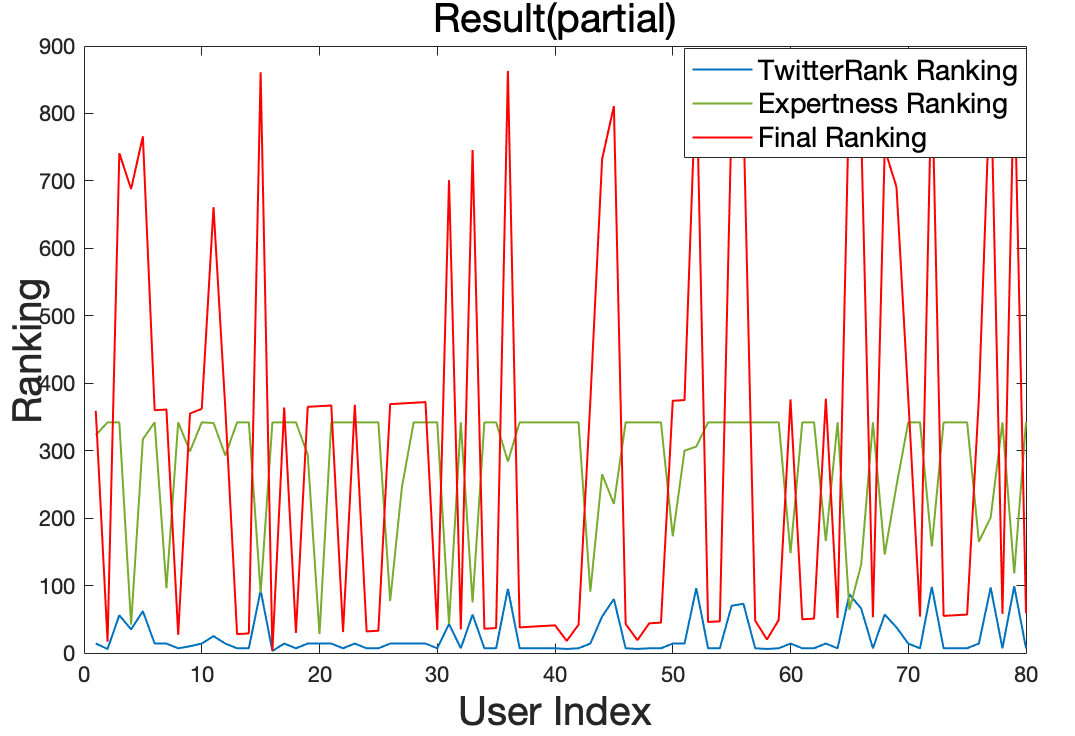
\includegraphics[width=0.8\linewidth]{4.png}
	\caption{Final Rank for $\alpha = 1$}
	\label{co10}
\end{figure} 

We can see from above that the final rank has the exact shape with the TwitterRank ranking, as $\alpha = 1$. Here, user influence ranking is not affected by their expertness.\\

\subsubsection{When $\alpha = $ 0.5}~\\
\indent The graph of the final ranking with $\alpha = 0.5$ is shown below.\par

\begin{figure}[htb]  
	\centering                       
	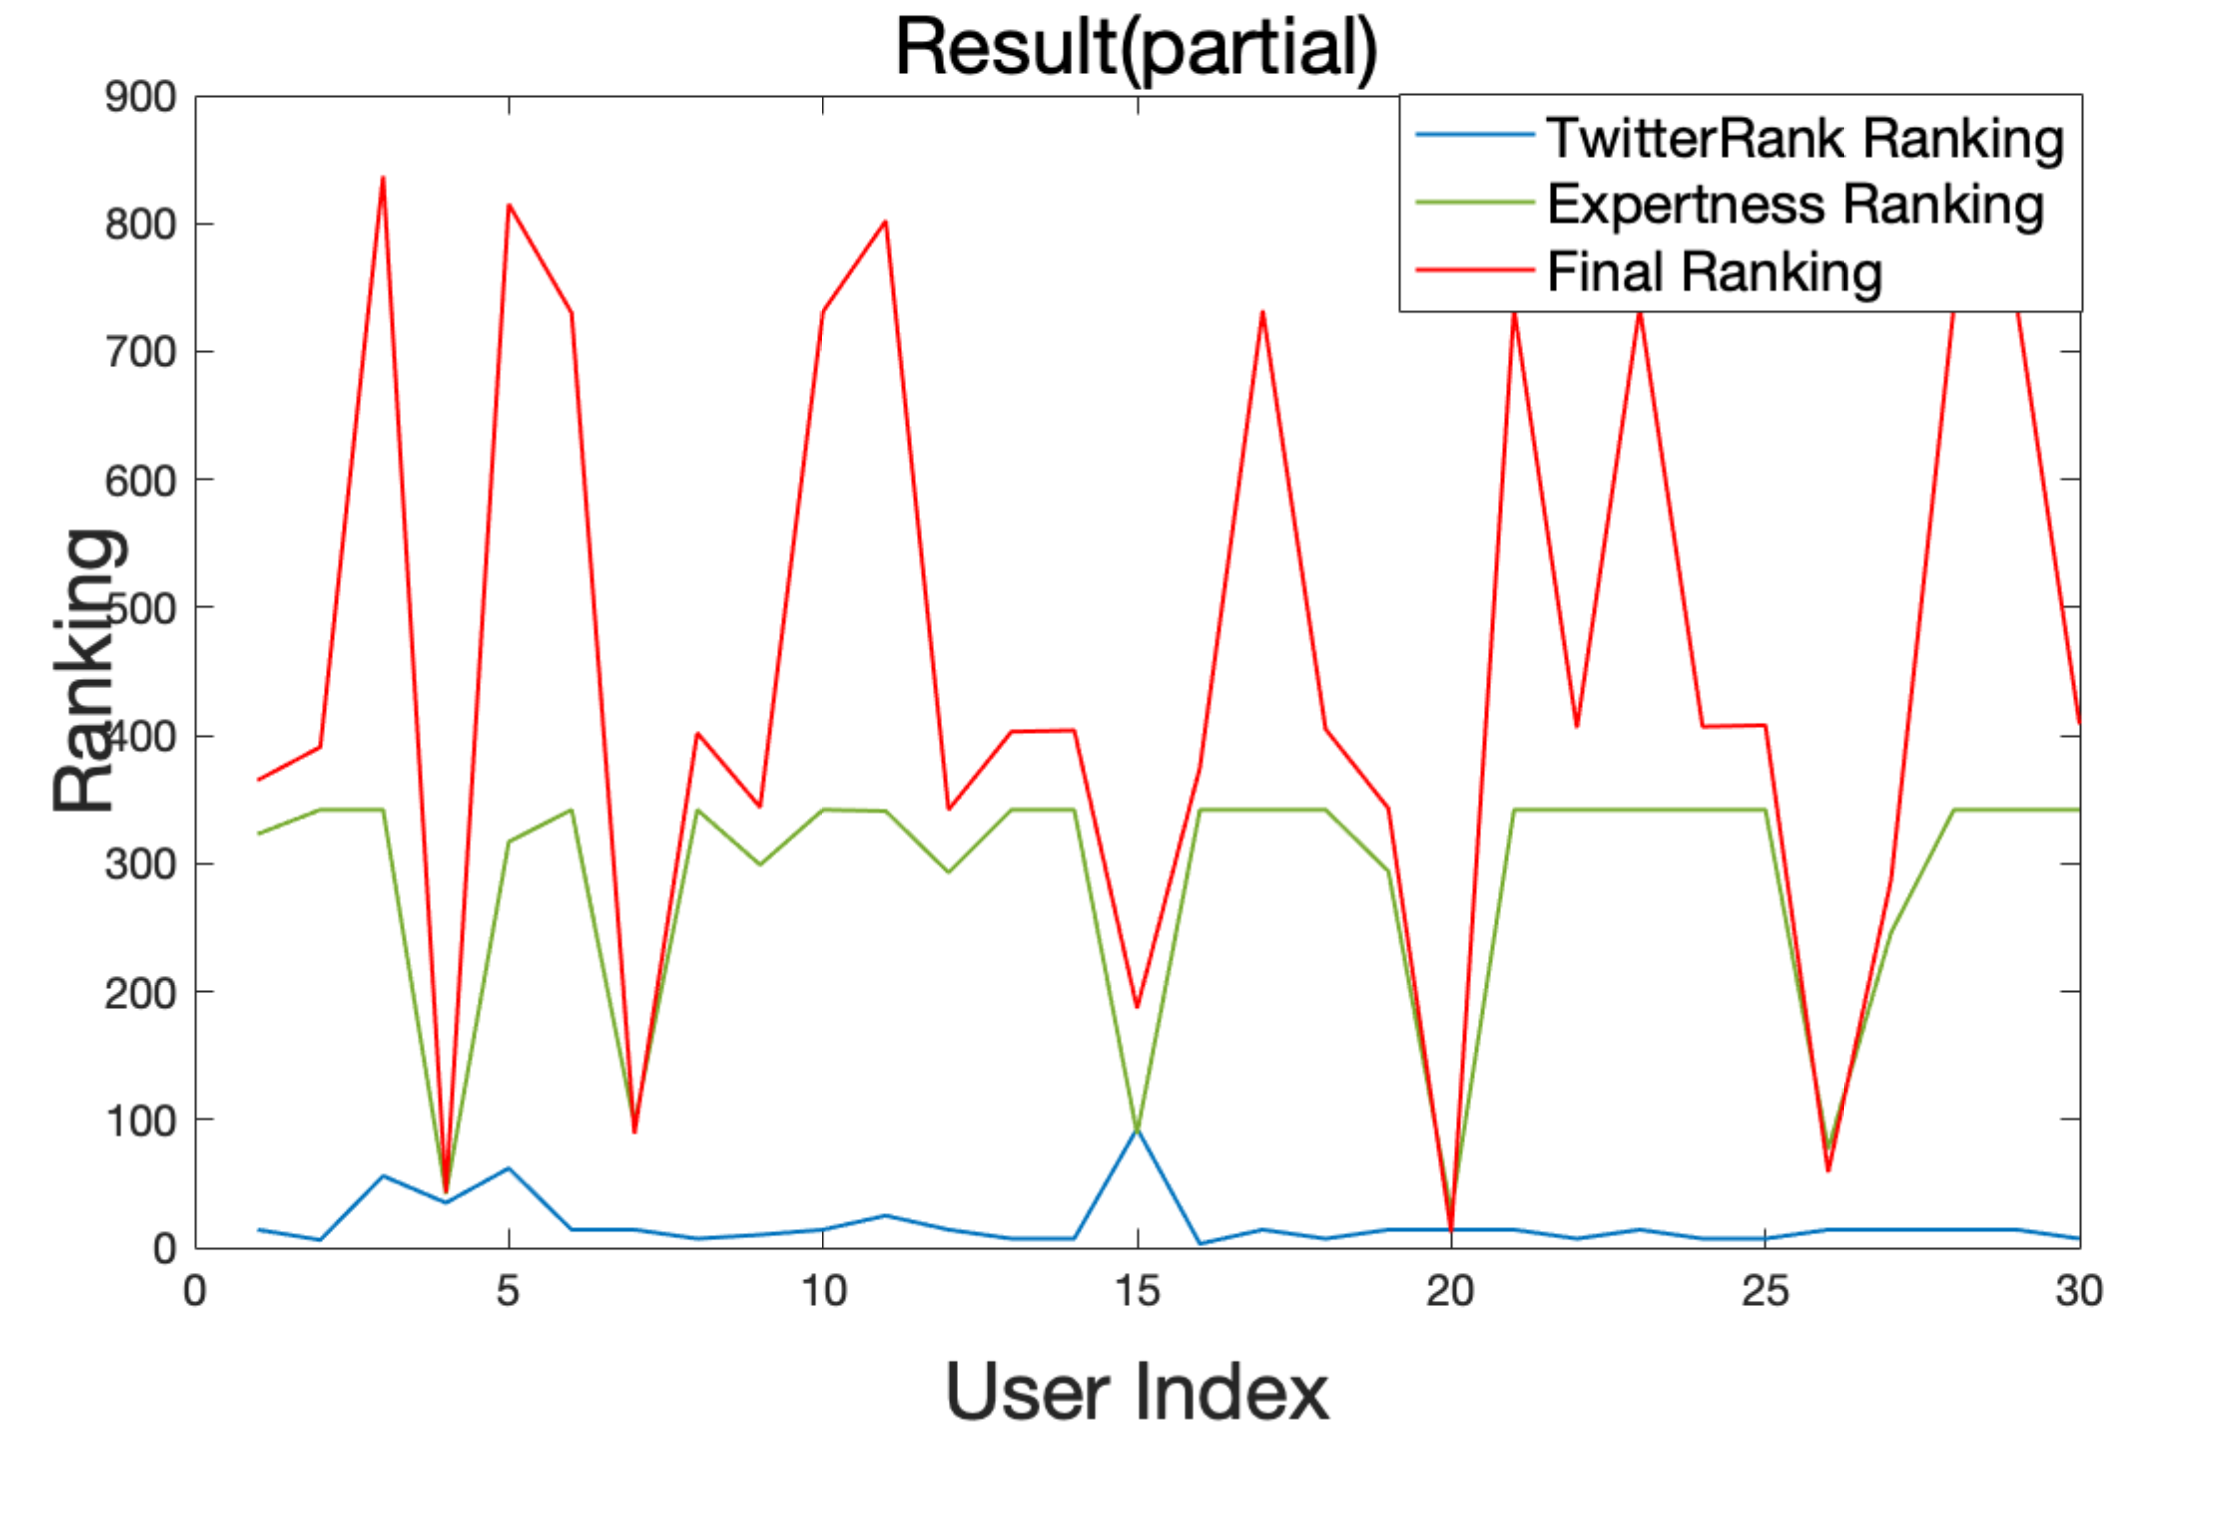
\includegraphics[width=0.8\linewidth]{5.png}
	\caption{Final Rank for $\alpha = 0.5$}
	\label{co05}
\end{figure} 

In this graph, we can find 4 kinds of combinations of two rankings: 

\begin{itemize}
	\item high TwitterRank + high Expertness = high final rank:\par
	e.g. user 20 has a final rank of 12 with TwitterRank 14 and Expertness 28.
	\item high TwitterRank + low Expertness = low final rank:\par
	e.g. user 56 has a final rank of 855 with TwitterRank 73 and Expertness 342 (ranked last).
	\item low TwitterRank + high Expertness = high final rank: \par
	e.g. user 65 has a final rank of 145 with TwitterRank 86 and Expertness 64.
	\item low TwitterRank + low Expertness = low final rank: \par
	e.g. user 82 has a final rank of 738 with TwitterRank 14 and Expertness 342 (ranked last).
\end{itemize}

To see how expertness ranking affect the final ranking, we compare user 56 and user 65, whose TwitterRank rankings are similar but with different expertness rankings. It is easy to find that although their importance regarding to degrees or topology are similar, the low expertness of user 56 significantly pulls down his final ranking which means expertness does carry weights on measuring user influence. And similar conclusion can be reached by comparing user 20 and user 82: TwitterRank ranking also has a influence in measurement. \par
Therefore, these comparisons verifies our assumption that both topology and special performance (expertness) can affect the measurement of node influence, and it is necessary to determine the weights each ranking carries in the final ranking combination.

\section{Conclusion}

This report analyzed the importance of Twitter users by employing two measures that capture different perspectives. We have implemented the TwitterRank method, which is an extension of the famous PageRank algorithm. We focus on the users who are interested and having commented the movies on 12 July, 2019. The TwitterRank method can form a network of them to detect the important users and they are ranked about topics. Retweets are driven to show another rank since the node importance may not result in the importance in certain topic. The number of retweets is qualified to show one's authority in the specific topic.

Focusing on the ranks from TwitterRank and retweets, we applied one famous voting method to balance and combine these two ranks. This Borda Count method results in the real rank of movies we focus on. By this method we can get the model to balance two rankings above and result in the wanted rank. The model is evaluated by analyzing the second group of data. The second group of data can lead to a rank based on this model and the rank has been compared to the real rank of movies' popularity. From the reasonable evaluation we have measured the performance of our model. The detailed analysis about our model has been discussed in the previous section.  


The study of influential nodes identification in general remains wide open, with many challenging issues and possible applications in the real world.









%\subsection{Figures and Tables}
%\paragraph{Positioning Figures and Tables} Place figures and tables at the top and 
%bottom of columns. Avoid placing them in the middle of columns. Large 
%figures and tables may span across both columns. Figure captions should be 
%below the figures; table heads should appear above the tables. Insert 
%figures and tables after they are cited in the text. Use the abbreviation 
%``Fig.~\ref{fig}'', even at the beginning of a sentence.
%
%\begin{table}[htbp]
%\caption{Table Type Styles}
%\begin{center}
%\begin{tabular}{|c|c|c|c|}
%\hline
%\textbf{Table}&\multicolumn{3}{|c|}{\textbf{Table Column Head}} \\
%\cline{2-4} 
%\textbf{Head} & \textbf{\textit{Table column subhead}}& \textbf{\textit{Subhead}}& \textbf{\textit{Subhead}} \\
%\hline
%copy& More table copy$^{\mathrm{a}}$& &  \\
%\hline
%\multicolumn{4}{l}{$^{\mathrm{a}}$Sample of a Table footnote.}
%\end{tabular}
%\label{tab1}
%\end{center}
%\end{table}

%\begin{figure}[htbp]
%\centerline{\includegraphics{1.png}}
%\caption{Example of a figure caption.}
%\label{fig}
%\end{figure}

%Figure Labels: Use 8 point Times New Roman for Figure labels. Use words 
%rather than symbols or abbreviations when writing Figure axis labels to 
%avoid confusing the reader. As an example, write the quantity 
%``Magnetization'', or ``Magnetization, M'', not just ``M''. If including 
%units in the label, present them within parentheses. Do not label axes only 
%with units. In the example, write ``Magnetization (A/m)'' or ``Magnetization 
%\{A[m(1)]\}'', not just ``A/m''. Do not label axes with a ratio of 
%quantities and units. For example, write ``Temperature (K)'', not 
%``Temperature/K''.


%\section*{Acknowledgment}
%
%The preferred spelling of the word ``acknowledgment'' in America is without 
%an ``e'' after the ``g''. Avoid the stilted expression ``one of us (R. B. 
%G.) thanks $\ldots$''. Instead, try ``R. B. G. thanks$\ldots$''. Put sponsor 
%acknowledgments in the unnumbered footnote on the first page.

%\section*{References}
%
%
%For papers published in translation journals, please give the English 
%citation first, followed by the original foreign-language citation \cite{b6}.

\begin{thebibliography}{00}
\bibitem{b1} Katz, E., Lazarsfeld, P. F., \& Roper, E. (2017). Personal influence: The part played by people in the flow of mass communications. Routledge.

\bibitem{b2} Cha, M., Haddadi, H., Benevenuto, F., \& Gummadi, K. P. (2010, May). Measuring user influence in twitter: The million follower fallacy. In fourth international AAAI conference on weblogs and social media.

\bibitem{b3} Kulshrestha, J., Kooti, F., Nikravesh, A., \& Gummadi, K. P. (2012, May). Geographic dissection of the twitter network. In Sixth International AAAI Conference on Weblogs and Social Media. 

\bibitem{b4} Weng, J., Lim, E. P., Jiang, J., \& He, Q. (2010, February). Twitterrank: finding topic-sensitive influential twitterers. In Proceedings of the third ACM international conference on Web search and data mining (pp. 261-270). ACM.

\bibitem{b5} Kwak, H., Lee, C., Park, H., \& Moon, S. (2010, April). What is Twitter, a social network or a news media?. In Proceedings of the 19th international conference on World wide web (pp. 591-600). AcM.

\bibitem{b6} Welch, M. J., Schonfeld, U., He, D., \& Cho, J. (2011, February). Topical semantics of twitter links. In Proceedings of the fourth ACM international conference on Web search and data mining (pp. 327-336). ACM.


\bibitem{b7} Ghosh, S., Viswanath, B., Kooti, F., Sharma, N. K., Korlam, G., Benevenuto, F., ... \& Gummadi, K. P. (2012, April). Understanding and combating link farming in the twitter social network. In Proceedings of the 21st international conference on World Wide Web (pp. 61-70). ACM.
\end{thebibliography}


\end{document}
